\subsection{Scaling Violations in parton densities}

Much smaller $Q^2$ lever arm than in the unpolarized case.

\begin{figure}
  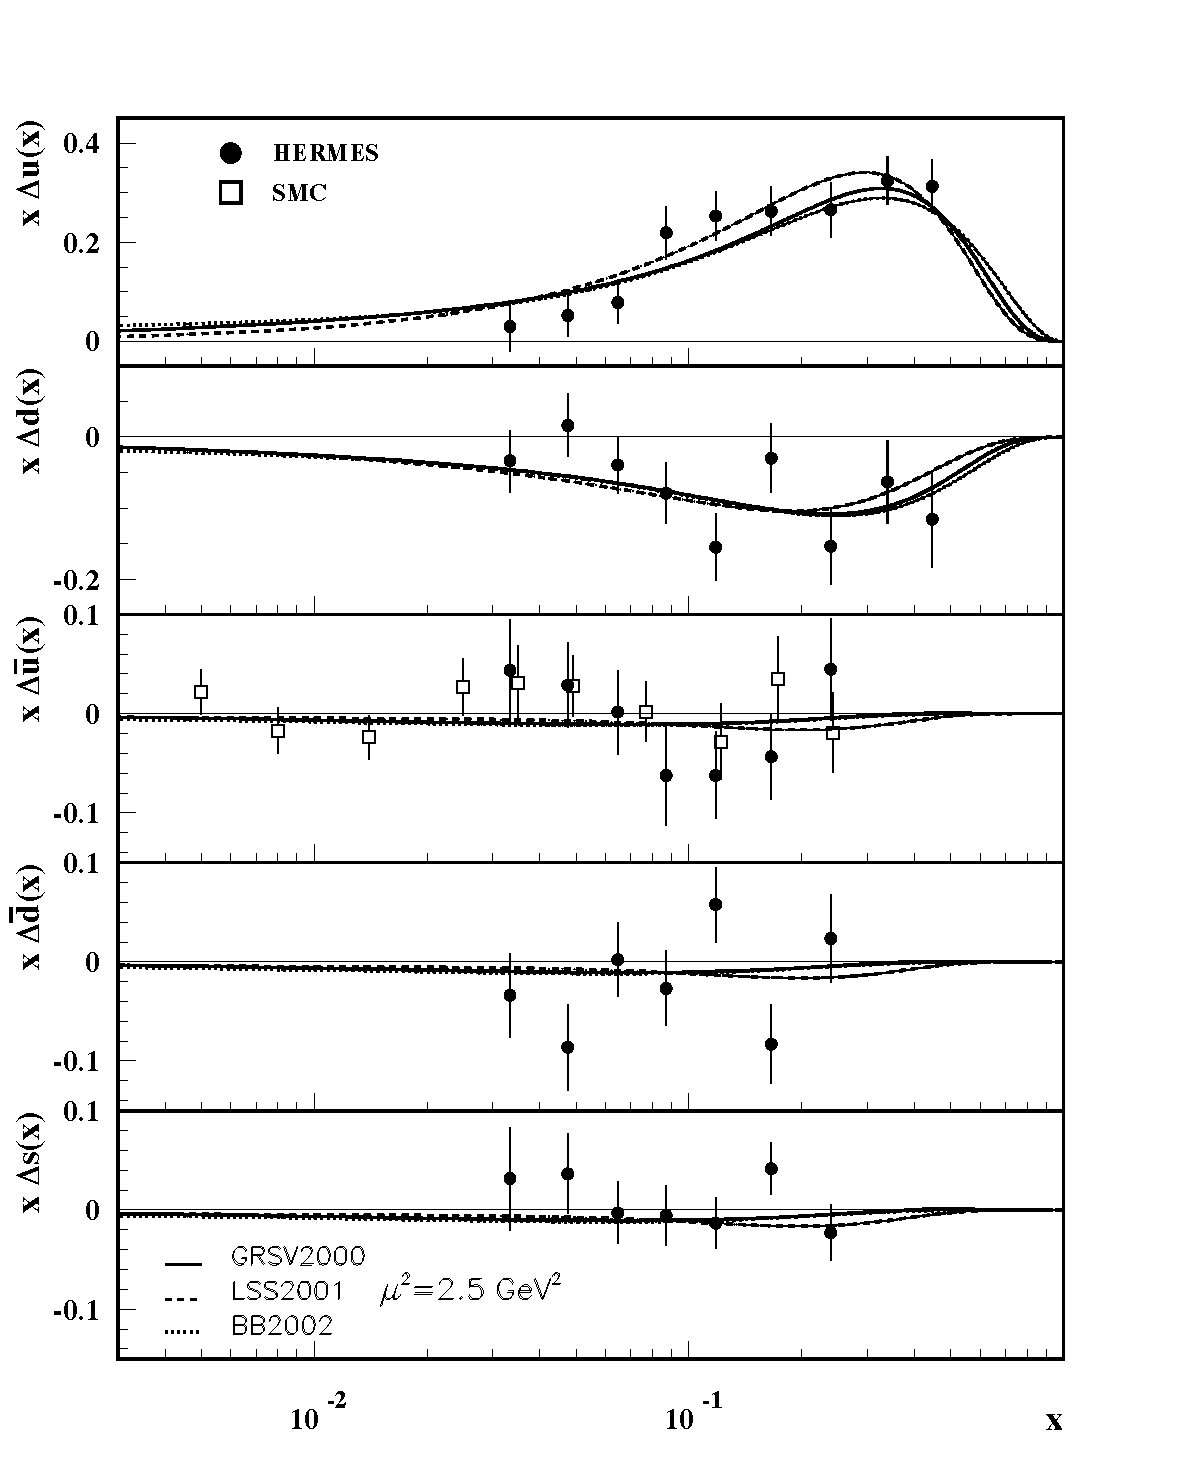
\includegraphics[width=1.0\textwidth]{figures/pol_pdf_5}
  \caption{from the Particle Data Group \cite{Amsler:2008zzb}.  Data points are SIDIS measurements using positron (HERMES) and muon (SMC).  SMC results extracted assuming $\Delta \bar u(x) = \Delta \bar d(x)$}
  \label{fig:pol_pdf_5}
\end{figure}

\begin{figure}
  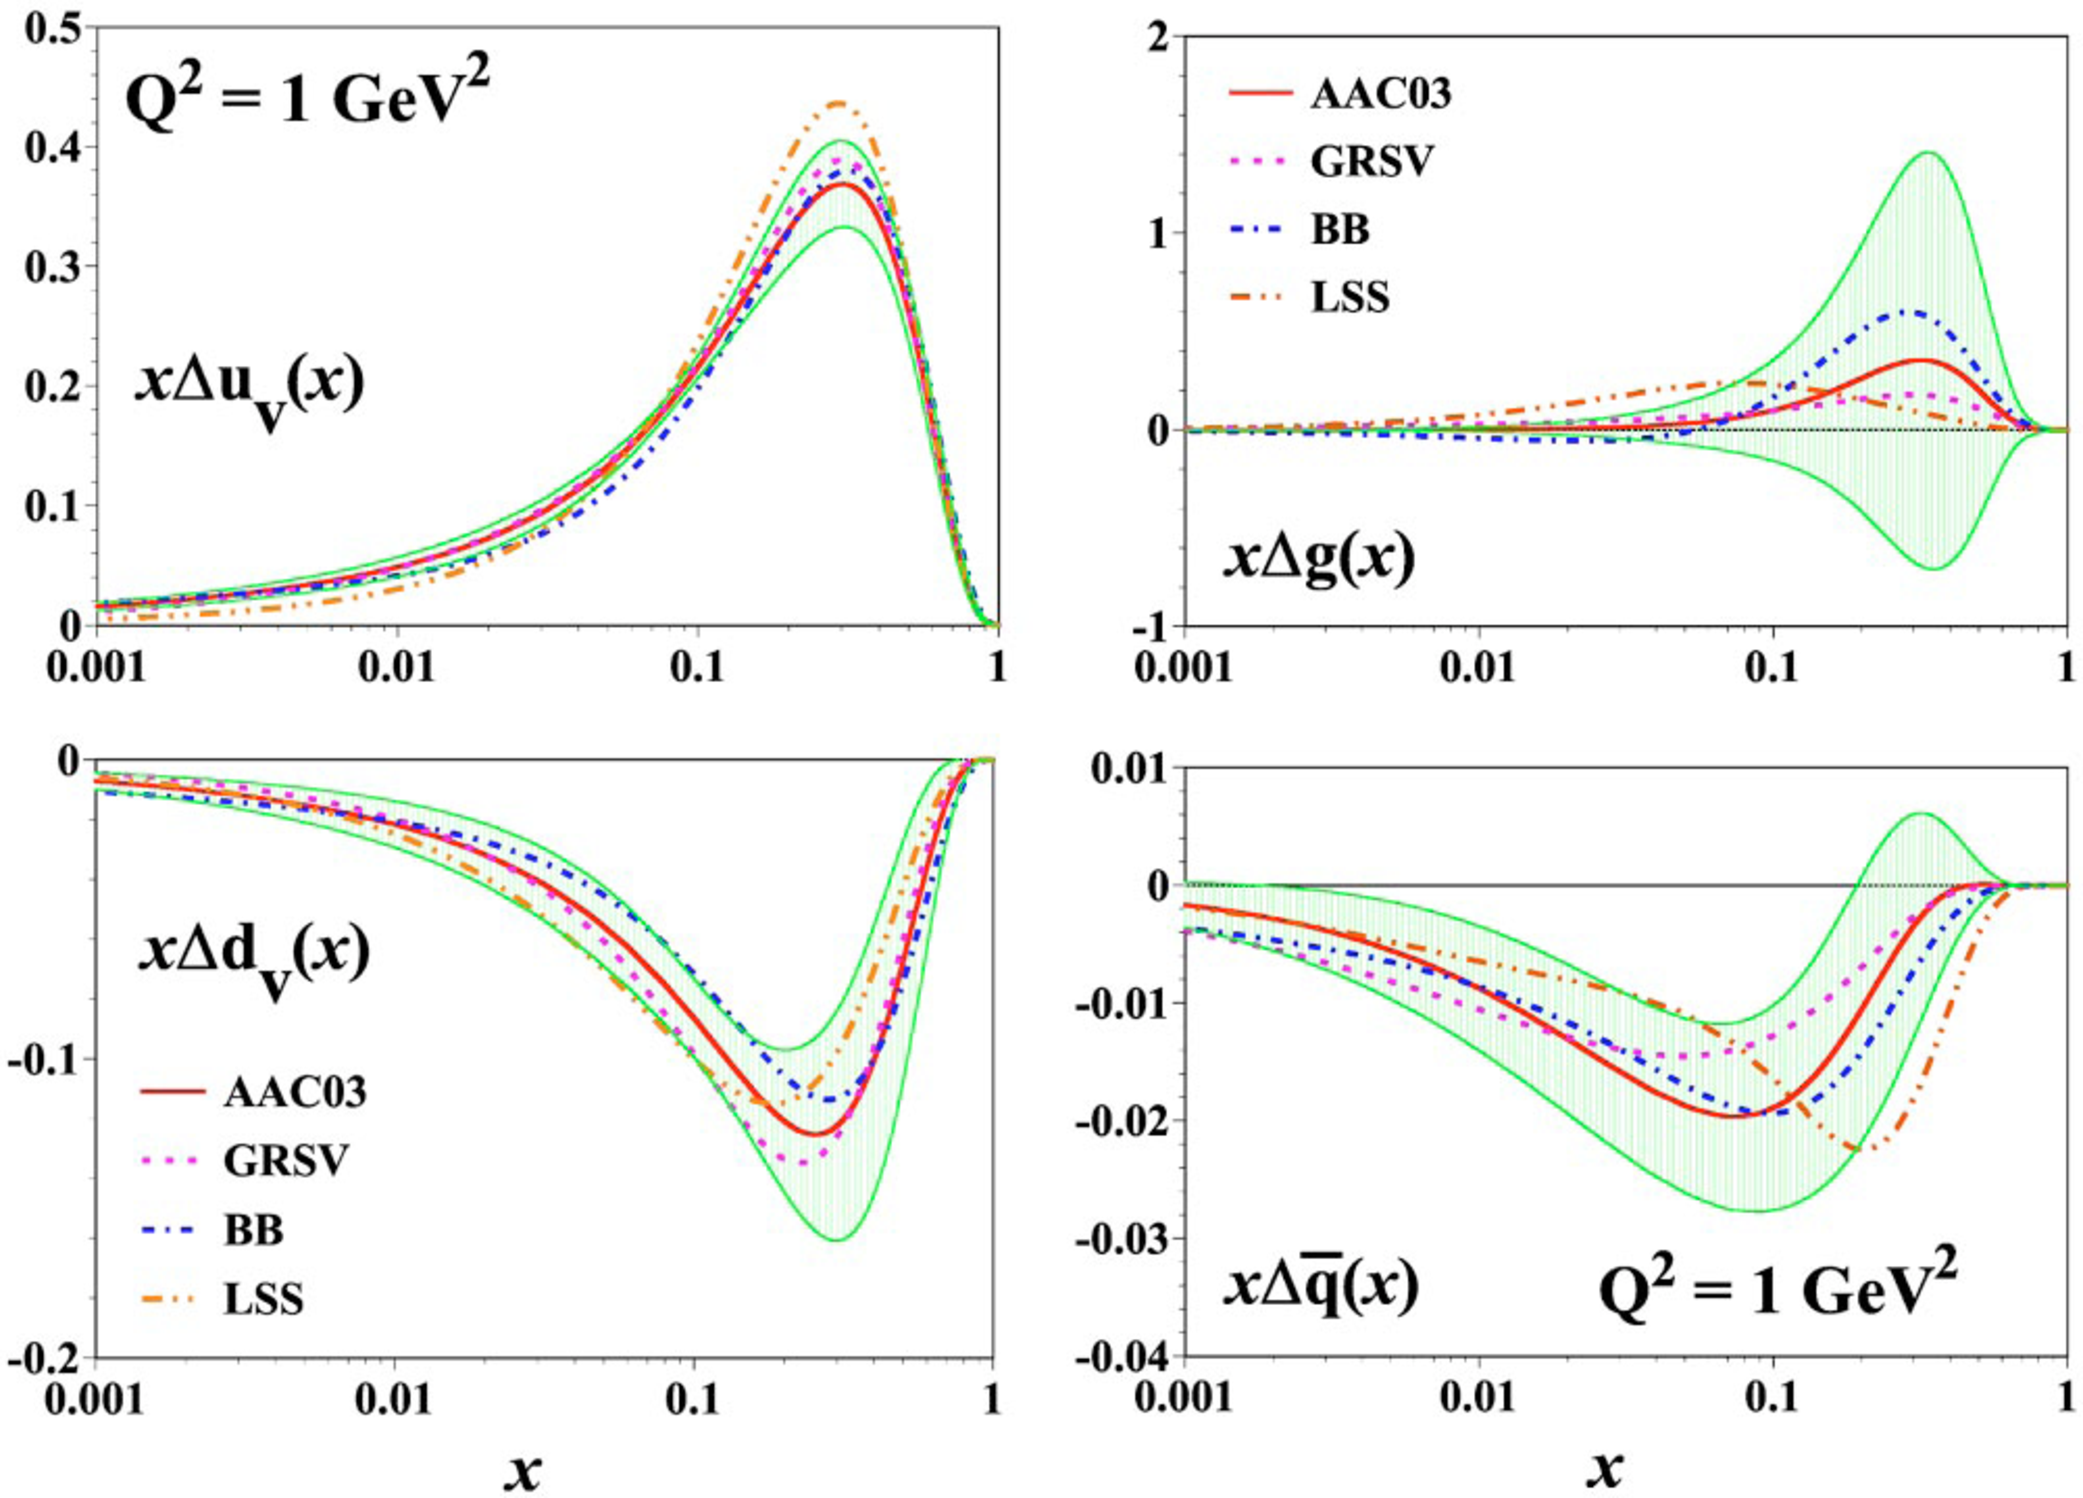
\includegraphics[width=1.0\textwidth]{figures/aac03}
  \caption{\cite{Hirai:2003pm}  BB \cite{Bluemlein:2002be} uses ISET=3, LSS \cite{Leader:2001kh} uses $\bar{MS}$, GRSV \cite{Gluck:2000dy} uses STD.  But this is of course \textit{not} the most recent polarized PDF analysis using only DIS and SIDIS data.  My best guess at that is \cite{Leader:2006xc}}
\end{figure}

\begin{figure}
  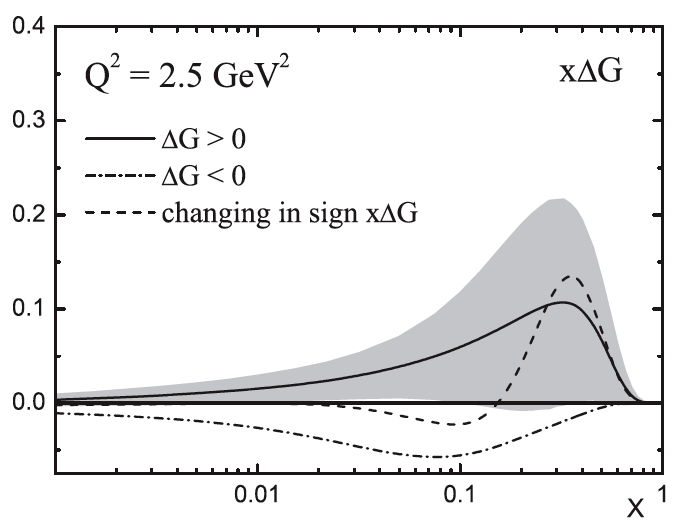
\includegraphics[width=1.0\textwidth]{figures/lss06_deltag}
  \caption{Newest $\Delta g(x)$ using only DIS and SIDIS data that I'm aware of. \cite{Leader:2006xc}}
\end{figure}

Need to understand what constraints go into positive/negative/sign-changing $\Delta g(x)$ parameterizations.
